% !TEX encoding = UTF-8
% !TEX TS-program = pdflatex
% !TEX root = ../tesi.tex

%**************************************************************
\chapter{Analisi dei requisiti}
\label{cap:analisi-requisiti}
%**************************************************************

\intro{In questo capitolo verranno elencati i casi d'uso delle funzionalità implementate con i relativi requisiti ed i loro tracciamento}\\

\section{Casi d'uso}

Per lo studio dei casi d'uso del prodotto creato sono stati creati dei diagrammi.
Questi diagrammi, detti appunto dei casi d'uso (in inglese \emph{Use Case Diagram}), sono diagrammi di tipo \gls{uml} dedicati alla descrizione del sistema e delle funzioni o servizi offerti da un esso, e come gli utilizzatori interagiscono con esso.\\
Lo strumento utilizzato per la realizzazione di tali diagrammi è StarUML, uno dei software più noti per la creazione di vari tipi di diagrammi utili alla progettazione architetturale di un prodotto software.

\subsection{Attori dei casi d'uso}
Dopo un'attenta analisi ho concluso che per le funzionalità offerte sono presenti unicamente attori primari, in quanto non ci sono collegamenti con alcun framework o libreria esterna.
Di conseguenza i possibili attori dei casi d'uso analizzati sono i seguenti attori primari:
\begin{itemize}
	\item utente non autenticato
	\item utente autenticato
\end{itemize}
\begin{figure}[H] 
	\centering 
	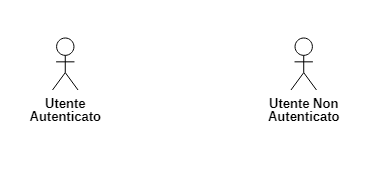
\includegraphics[width=0.9\columnwidth]{usecase/attori} 
	\caption{Attori dei casi d'uso}
\end{figure}

\begin{usecase}{1}{Registrazione}\\
	\begin{figure}[H] 
		\centering 
		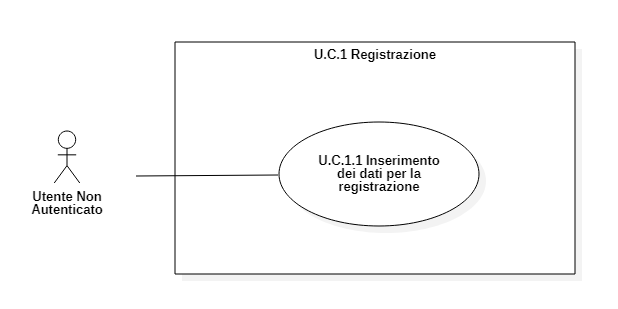
\includegraphics[width=0.9\columnwidth]{usecase/UC1.1} 
		\caption{U.C1.1 Inserimento dei dati per la registrazione}
	\end{figure}
\usecaseactors{Utente non autenticato}
\usecasepre{L'utente non è ancora presente nei registri del sistema}
\usecasedesc{L'utente accede all'applicazione e naviga fino alla pagina di registrazione. L'utente inserisce i dati necessari e li conferma, questo porta l'utente a possedere un account nel sistema}
\usecasepost{L'utente risulta presente nei registri del sistema ed è autenticato nella piattaforma}
\end{usecase}

\begin{usecase}{1.1}{Inserimento dei dati per la registrazione}
		\begin{figure}[H] 
		\centering 
		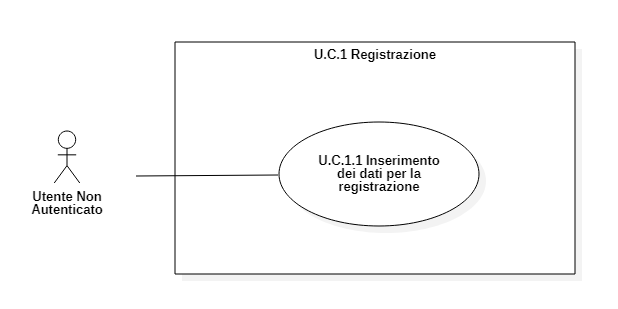
\includegraphics[width=0.9\columnwidth]{usecase/UC1.1} 
		\caption{U.C1.1 Inserimento dei dati per la registrazione}
	\end{figure}
\usecaseactors{Utente non autenticato}
\usecasepre{L'utente non autenticato si trova nella pagina di navigazione}
\usecasedesc{L'utente non autenticato compila i campi nel seguente modo:
\begin{itemize}
	\item Inserimento del nome (U.C1.1.1)
	\item Inserimento del cognome (U.C1.1.2)
	\item Inserimento dell'email (U.C1.1.3)
	\item Inserimento della password (U.C1.1.4)
	\item Inserimento della conferma della password (U.C1.1.5)
	\item Inserimento dell'anno di nascita (U.C1.1.6)
	\item Inserimento del Wallet Address (U.C.1.1.7)
\end{itemize}
DA SISTEMARE PER IL PUNTO SCEMO}
\usecasepost{L'utente ha completato la compilazione dei campi e può procedere con la registrazione}
\end{usecase}

\begin{usecase}{1.1.1}{Inserimento del nome}
\usecaseactors{Utente non autenticato}
\usecasepre{L'utente non è autenticato e non ha compilato questo campo}
\usecasedesc{L'utente non autenticato inserisce il proprio nome}
\usecasepost{L'utente ha inserito il nome}
\end{usecase}

\begin{usecase}{1.1.2}{Inserimento del cognome}
\usecaseactors{Utente non autenticato}
\usecasepre{L'utente non è autenticato e non ha compilato questo campo}
\usecasedesc{L'utente non autenticato inserisce il proprio cognome}
\usecasepost{L'utente ha inserito il cognome}
\end{usecase}

\begin{usecase}{1.1.3}{Inserimento dell'email}
\usecaseactors{Utente non autenticato}
\usecasepre{L'utente non è autenticato e non ha compilato questo campo}
\usecasedesc{L'utente non autenticato inserisce la sua email}
\usecasepost{L'utente ha inserito l'email}
\end{usecase}

\begin{usecase}{1.1.4}{Inserimento della password}
\usecaseactors{Utente non autenticato}
\usecasepre{L'utente non è autenticato e non ha compilato questo campo}
\usecasedesc{L'utente non autenticato inserisce la sua password}
\usecasepost{L'utente ha inserito la password}
\end{usecase}

\begin{usecase}{1.1.5}{Inserimento della conferma della password}
\usecaseactors{Utente non autenticato}
\usecasepre{L'utente non è autenticato e non ha compilato questo campo}
\usecasedesc{L'utente non autenticato inserisce la conferma della password}
\usecasepost{L'utente ha inserito la conferma della password}
\end{usecase}

\begin{usecase}{1.1.6}{Inserimento dell'anno di nascita}
\usecaseactors{Utente non autenticato}
\usecasepre{L'utente non è autenticato e non ha compilato questo campo}
\usecasedesc{L'utente non autenticato inserisce il proprio anno di nascita}
\usecasepost{L'utente ha inserito l'anno di nascita}
\end{usecase}

\begin{usecase}{1.1.7}{Inserimento del Wallet Address}
\usecaseactors{Utente non autenticato}
\usecasepre{L'utente non è autenticato e non ha compilato questo campo}
\usecasedesc{L'utente non autenticato inserisce il Wallet Address}
\usecasepost{L'utente ha inserito il Wallet Address}
\end{usecase}

\begin{usecase}{2}{Login}
\usecaseactors{Utente non autenticato}
\usecasepre{L'utente non è autenticato ma è presente nei registri di sistema}
\usecasedesc{L'utente accede all'applicazione e naviga fino alla pagina di login. L'utente inserisce i dati necessari e li conferma, questo porta l'utente ad autenticarsi nel sistema.}
\usecasepost{L'utente risulta autenticato nella piattaforma}
\end{usecase}

\begin{usecase}{2.1}{Inserimento dei dati per il login}
	\begin{figure}[H] 
		\centering 
		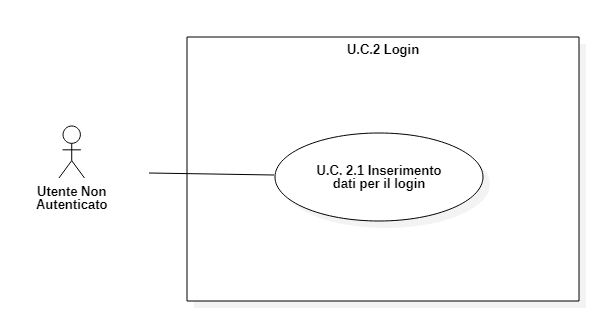
\includegraphics[width=0.9\columnwidth]{usecase/UC2.1} 
		\caption{U.C1.1 Inserimento dei dati per la registrazione}
	\end{figure}
\usecaseactors{Utente non autenticato}
\usecasepre{}
\usecasedesc{}
\usecasepost{}
\end{usecase}

\section{Tracciamento dei requisiti}

Come risultato di un'attenta analisi dei requisiti e i relativi casi d'uso effettuata sul progetto sono stati individuati diversi requisiti. Questi sono stati suddivisi per classificazione e tipologia, per questo motivo si utilizza un codice identificativo per distinguerli che è così strutturato:
\begin{center}
	\textbf{R[classificazione][tipologia][codice]}
\end{center}
La descrizione del codice è la seguente:
\begin{itemize}
	\item \textbf{R}: acronimo per Requisito;
	\item \textbf{classificazione}: individua la classificazione del requisito e può essere:
	\begin{itemize}
		\item [F =] funzionale
		\item [Q =] qualitativo
		\item [V =]  di vincolo
	\end{itemize}
	\item \textbf{tipologia}: individua la tipologia del requisito e può essere:
	\begin{itemize}
		\item [O =] obbligatorio
		\item [D =] desiderabile
		\item [F =] facoltativo
	\end{itemize}
\end{itemize}

Nelle sezioni seguenti sono riassunti i requisiti ed il loro tracciamento con i casi d'uso delineati in fase di analisi.

\begin{table}%
\caption{Tabella del tracciamento dei requisti funzionali}
\label{tab:requisiti-funzionali}
\begin{tabularx}{\textwidth}{lXl}
\hline\hline
\textbf{Requisito} & \textbf{Descrizione} & \textbf{Use Case}\\
\hline
RFO1 & L'interfaccia permette di effettuare la registrazione al sito & UC1 \\
\hline
RFO2 & L'interfaccia permette di effettuare il login al sito & UC2 \\
\hline
\end{tabularx}
\end{table}%

\begin{table}%
\caption{Tabella del tracciamento dei requisiti qualitativi}
\label{tab:requisiti-qualitativi}
\begin{tabularx}{\textwidth}{lXl}
\hline\hline
\textbf{Requisito} & \textbf{Descrizione} & \textbf{Use Case}\\
\hline
RQD-1    & Le prestazioni del simulatore hardware deve garantire la giusta esecuzione dei test e non la generazione di falsi negativi & - \\
\hline
\end{tabularx}
\end{table}%

\begin{table}%
\caption{Tabella del tracciamento dei requisiti di vincolo}
\label{tab:requisiti-vincolo}
\begin{tabularx}{\textwidth}{lXl}
\hline\hline
\textbf{Requisito} & \textbf{Descrizione} & \textbf{Use Case}\\
\hline
RVO-1    & La libreria per l'esecuzione dei test automatici deve essere riutilizzabile & - \\
\hline
\end{tabularx}
\end{table}%